\section{Priors and normalization}

In this section we will add the priors in the parameter and normalize the data to see how it can improve the result on the trained methods.

The priors are, for opencv, argements given to the training model to specify the classes repartition within the data, here 84\% of non ad and 16\% of ads.

Normalizing the data can improve results depending on the method used. For instance for the svm it can help improving the results by "giving the same improtance to each point in the data vector". Meaning no value will be overpowerful over the others (range from -30 to 30 aginst range from -1 to 1).

\subsection{SVM}

Here we still use the autotrain method still with 2 folds. Again here the main goal is to test the effects of normalization and priors on the dataset, not the get the best parameter with a crossvalidation.

\subsubsection{linear}

The first type of model used was the linear one. The stopping criteria was of either a 1000000 iterations or 0.001 for epsilon.

Results :
\begin{itemize}
  \item Correct classification : 90.37\%;
  \item Wrong classification : 9.632\%;
  \item False positive non ad : 8.78\%;
  \item False positive ad : 0.85\%.
\end{itemize}

The final parameters were the following ones :
\begin{itemize}
  \item C : 0.1.
\end{itemize}

\subsubsection{Polynomial}

For this one, the number of itertion was reduced to 1000 because it was taking too much time.

Results :
\begin{itemize}
  \item Correct classification : 88.67\%;
  \item Wrong classification : 11.33\%;
  \item False positive non ad : 10.2\%;
  \item False positive ad : 1.13\%.
\end{itemize}

The final parameters were the following ones :
\begin{itemize}
  \item degree : 0.07
  \item gamma : 0.00225;
  \item coef0 : 1.4;
  \item C : 321.5.
\end{itemize}

\subsubsection{Radial Basis Function}

Since the result on the first model were not good enough I tried an other one, the polynomial one. As shown after the results were much better.

Results :
\begin{itemize}
  \item Correct classification : 89.52\%;
  \item Wrong classification : 10.48\%;
  \item False positive non ad : 9.92\%;
  \item False positive ad : 0.57\%.
\end{itemize}

The final parameters were the following ones :
\begin{itemize}
  \item gamma : 0.00015;
  \item C : 62.5.
\end{itemize}

\subsubsection{Sigmoid}

Since the result on the first model were not good enough I tried an other one, the polynomial one. As shown after the results were much better.

Results :
\begin{itemize}
  \item Correct classification : 83.85\%;
  \item Wrong classification : 16.15\%;
  \item False positive non ad : 16.15\%;
  \item False positive ad : 0\%.
\end{itemize}

The final parameters were the following ones :
\begin{itemize}
  \item gamma : 0.00001;
  \item coef0 : 0.1;
  \item C : 0.1.
\end{itemize}

\subsection{Neural Network}
For the neural network, the layers used are as follow :
  \begin{itemize}
    \item input layer, 1558, the number of point in the vector inputs;
    \item output layer, 2 outputs the number of class;
    \item hidden layer;
  \end{itemize}

The final number of cells within the hidden layer was of 90;

  Results :
  \begin{itemize}
    \item Correct classification : 88.67\%;
    \item Wrong classification : 11.33\%;
    \item False positive non ad : 6.23\%;
    \item False positive ad : 5.10\%.
  \end{itemize}

  \begin{figure}[h]
   \centering
   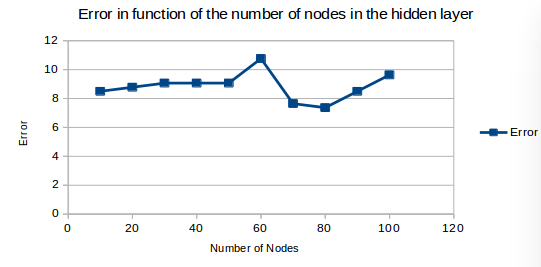
\includegraphics[scale=0.5]{../images/NNPO.png}
   \caption{Class diagram}
  \end{figure}

\subsection{Random forest}
The parameters used for the random forest are the following :
  \begin{itemize}
    \item number of variable randomly selected sqrt(n) (usually the best number);
  \end{itemize}
Results :
\begin{itemize}
  \item Correct classification : 87.25\%;
  \item Wrong classification : 12.75\%;
  \item False positive non ad : 12.46\%;
  \item False positive ad : 0.2833\%.
\end{itemize}

\begin{figure}[h]
 \centering
 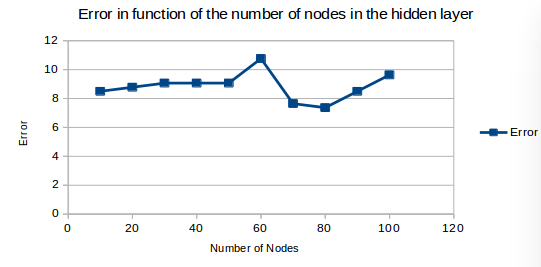
\includegraphics[scale=0.5]{../images/NNPO.png}
 \caption{Class diagram}
\end{figure}
500
